% Created 2021-03-29 Mon 20:21
% Intended LaTeX compiler: xelatex
\documentclass[letterpaper,11pt]{article}
%% Margins
\usepackage{geometry}
\geometry{verbose,margin=1.5in}
\setlength\parindent{0pt}
\linespread{1.1}
%% Typesetting
\usepackage[stretch=10,babel=true]{microtype} % better typesetting. works w/ pdftex, not latex.
%% \usepackage[english]{babel} % manages hyphenation patterns
%% \usepackage{polyglossia} \setdefaultlanguage{english} % babel replacement for XeLaTex.
\usepackage{csquotes} % Context sensitive quotation facilities
%% Biblio
\usepackage[natbib=true, sorting=ynt, backend=biber, minbibnames=3, maxbibnames=3, doi=false, isbn=false, style=authoryear]{biblatex}
\addbibresource{~/Zotero/myref.bib}
\AtEveryBibitem{\clearfield{note}}
\AtEveryBibitem{\clearfield{month}}
\AtEveryBibitem{\clearfield{day}}
\AtEveryBibitem{\clearfield{eprint}}
%% Math
\usepackage{amsmath} % \declareMathOperator
\usepackage[mathbf=sym]{unicode-math}
%% \usepackage{cool} % for math operators & symbols e.g. partial diff
\usepackage{mathtools} % for math aligning & spacing
\usepackage{physics} % derivative, dx, operators
\usepackage{cancel}
\allowdisplaybreaks % Allow new page within align
%% Font
\usepackage{kotex}
\setmainfont{XITS}
\setmathfont{XITS Math} % \boldsymbol works
\setmathfont[range={\mathcal,\mathbfcal},StylisticSet=1]{XITS Math}
\usepackage[unicode,colorlinks]{hyperref}

\usepackage{graphicx}
\usepackage{subfigure}
\usepackage{grffile} % Extended file name support for graphics (legacy package)
\usepackage{float} % Fix figures and tables by [H]
\usepackage{longtable}
\usepackage{wrapfig}
\usepackage{rotating}
\usepackage[normalem]{ulem}
\usepackage{textcomp}
\usepackage{capt-of}
\author{Jonghyun Yun}
\date{\today}
\title{\textit{[2021-03-29 Mon] } Discussion}
\hypersetup{
 pdfauthor={Jonghyun Yun},
 pdftitle={\textit{[2021-03-29 Mon] } Discussion},
 pdfkeywords={},
 pdfsubject={},
 pdfcreator={Emacs 27.1 (Org mode 9.5)}, 
 pdflang={English}}
\begin{document}

\maketitle

\section*{\textit{[2021-03-29 Mon] } Updates}
\label{sec:orgfb91d4a}
\begin{itemize}
\item Code debugging finished for MCMC sampler (\(\beta, \theta\))
\item \(\beta_{ic}\) is non-identifiable, dropped.
\item New posterior analysis is ready to look.
\item piecewise approximation segment number: back to 5 (was 2).
\begin{itemize}
\item at a small \# of segments, the latent space doesn't improve the fit to chessB data (log-loss).
\end{itemize}
\item 유월 서브미션 목표!!
\end{itemize}
\section*{Log-loss}
\label{sec:org04bec69}
Given the survival time \(t\) and MCMC samples, the conditional probability of ``correct'' response is estimated as
\[
\hat p_{ik}^{(l)}(t) = \frac{h_{i1}^{(l)}(t)}{h_{i1}^{(l)}(t) + h_{i0}^{(l)}(t)},
\]
where \((l)\) denote the index of MCMC sample used to calculate the quantity.
We use \(Y_{ik} = 1\) to denote a correct response, and \(Y_{ik} = 0\) an incorrect response. Then, \(p_{ik}^{(l)}(t)\) can be served as the prediction probability of \(Y_{ik}\), which allows using classification performance metrics. For easiness of evaluation, we use the log-loss for item:

\[
-\frac{1}{N}
\sum_{k} \left\{ y_{ik} \log \hat p_{ik}^{(l)}(t) + (1-y_{ik}) \log (1 - \hat p_{ik}^{(l)})\right\}.
\]

\section*{Models}
\label{sec:org88b34bf}
\texttt{double pp} model:
the smaller distance, the faster process
\begin{align*}
h_{i1}(t) &= \lambda_{i1}(t) \exp(\theta_{k1} - \gamma_{1} ||z_{k1} - w_{i1}||) \\
h_{i0}(t) &= \lambda_{i0}(t) \exp(\theta_{k0} - \gamma_{0} ||z_{k0} - w_{i0}||) \\
\end{align*}

\texttt{np} model: the smaller distance, the more distinct process (in terms of speed).
\begin{align*}
h_{i1}(t) &= \lambda_{i1}(t) \exp(\theta_{k1} + \gamma ||z_{k} - w_{i}||) \\
h_{i0}(t) &= \lambda_{i0}(t) \exp(\theta_{k0} - \gamma ||z_{k} - w_{i}||) \\
\end{align*}

\section*{\(\gamma\) is non-identifiable, but it's ok to keep}
\label{sec:org918211b}
\texttt{np} model with \(\gamma = 1\).
\begin{align*}
h_{i1}(t) &= \lambda_{i1}(t) \exp(\theta_{k1} + ||z_{k} - w_{i}||) \\
h_{i0}(t) &= \lambda_{i0}(t) \exp(\theta_{k0} - ||z_{k} - w_{i}||) \\
\end{align*}
\begin{itemize}
\item priors on the latent space
\begin{align*}
\pi\left(\mathbf{z}_{j}\right) & \sim \mathrm{MVN}_{d}\left(0, I_{d}\right) \\
\pi\left(\mathbf{w}_{i}\right) & \sim \mathrm{MVN}_{d}\left(0, I_{d}\right) \\
\end{align*}
\item results (latent space structure) heavily depend on the prior variance (\(\sigma_{zw}\)) of \(z_{k}\) and \(w_{i}\).
\item we should let the data determine \(\sigma_{zw}\).
\end{itemize}

\section*{{\bfseries\sffamily KILL} fit the model}
\label{sec:orga265a6f}
\begin{itemize}
\item State ``KILL''       from ``TODO''       \textit{[2021-03-29 Mon 09:29] } \\
cannot do the model selection based on a non-identifiable parameter.
\end{itemize}
\begin{align*}
h_{i1}(t) &= \lambda_{i1}(t) \exp(\theta_{k1} + \gamma_{} ||z_{k} - w_{i}||) \\
h_{i0}(t) &= \lambda_{i0}(t) \exp(\theta_{k0} - \gamma_{} ||z_{k} - w_{i}||) \\
\end{align*}
\[
\gamma_{} \sim N(0,1)
\]

\section*{diffused priors?}
\label{sec:org891850c}
\begin{align*}
\pi\left(\lambda_{ic,j}\right) & \sim \operatorname{Gamma}\left(\text{mean} = \tilde \lambda_{ic,j}, \text{var} = C \cdot \tilde \lambda_{ic,j})\right) \\
\pi\left(\theta_{k} | \sigma^{2}\right) & \sim \mathrm{N}\left(0, \sigma^{2}\right) \\ \pi\left(\sigma^{2}\right) & \sim \operatorname{lnv}-\operatorname{Gamma}\left(a_{\sigma}, b_{\sigma}\right) \\
\pi\left(\mathbf{z}_{j}\right) & \sim \mathrm{MVN}_{d}\left(0, I_{d}\right) \\
\pi\left(\mathbf{w}_{i}\right) & \sim \mathrm{MVN}_{d}\left(0, I_{d}\right) \\
\pi(
\log \gamma) & \sim \mathrm{N}\left(\mu_{\gamma}, \tau_{\gamma}^{2}\right)
\end{align*}
\[C = 2, a_{\sigma}=0.0001, b_{\sigma}=0.0001, \mu_{\gamma}=0, \text { and } \tau_{\gamma}^{}=2\]
\subsection*[How to set \(\lambda\) priors]{How to set \(\lambda\) priors\hfill{}\textsc{ATTACH}}
\label{sec:org85b5ee2}
C=2, K\_j: number of segments, U\_j = 3rd quartile, k: k-th segment.
\begin{center}
\includegraphics[width=.9\linewidth]{/Users/yunj/org/.attach/ad/c42ad2-5845-4405-bed4-b640f540b3d9/_20210322_183639screenshot.png}
\end{center}
\section*{New results with unknown \(\gamma > 0\).}
\label{sec:org12f4918}
baseline model:
\begin{align*}
h_{i1}(t) &= \lambda_{i1}(t) \exp(\theta_{k1})\\
h_{i0}(t) &= \lambda_{i0}(t) \exp(\theta_{k0})\\
\end{align*}

\begin{center}
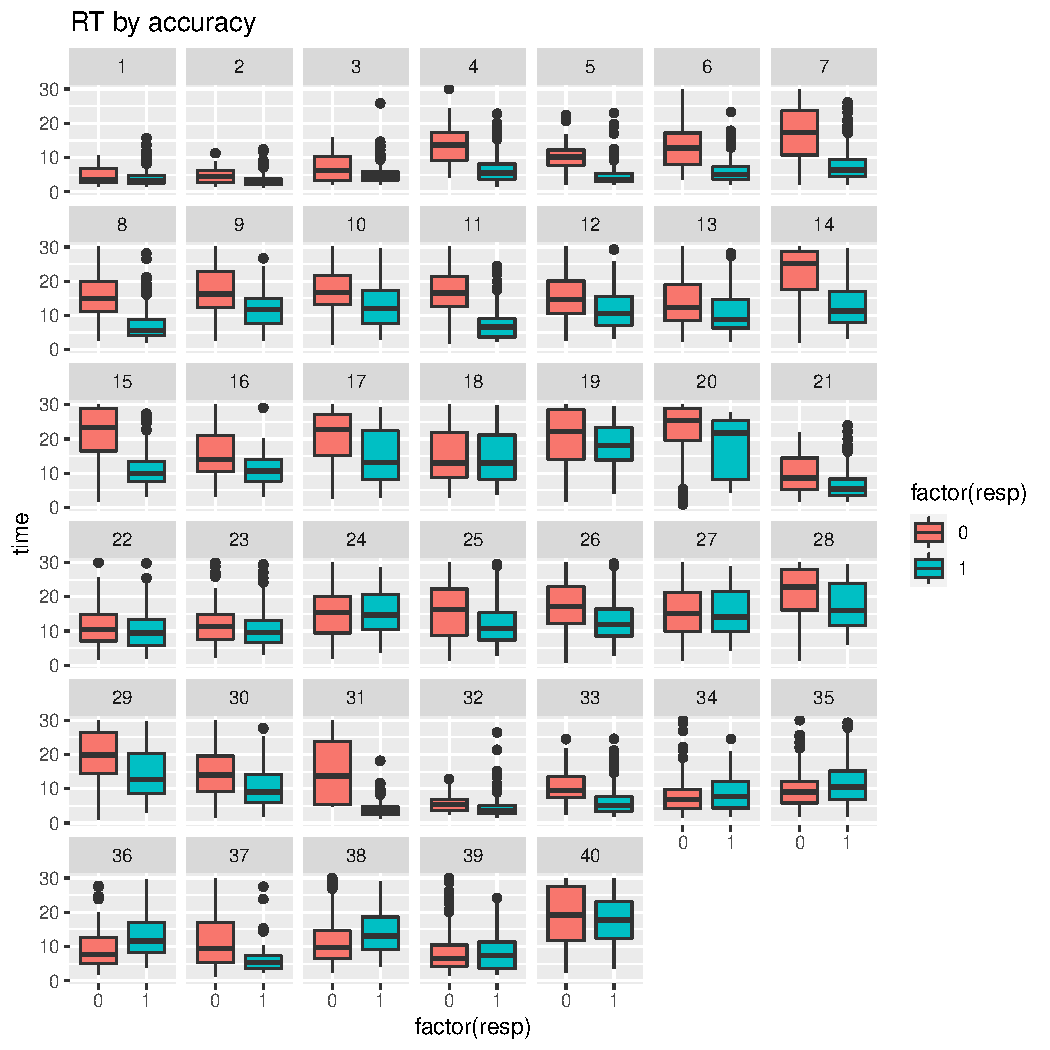
\includegraphics[width=.9\linewidth]{chessB_RTnACC.pdf}
\end{center}
\begin{center}
\begin{tabular}{l}
chessB\_no\_latent\_ncut5\_zero\_beta\_noinfo\_lc2\\
chessB\_double\_nn\_ncut5\_zero\_beta\_noinfo\_lc2\\
chessB\_double\_np\_ncut5\_zero\_beta\_noinfo\_lc2\\
chessB\_double\_pn\_ncut5\_zero\_beta\_noinfo\_lc2\\
chessB\_double\_pp\_ncut5\_zero\_beta\_noinfo\_lc2\\
chessB\_nn\_ncut5\_zero\_beta\_noinfo\_lc2\\
chessB\_np\_ncut5\_zero\_beta\_noinfo\_lc2\\
\textbf{chessB\_pn\_ncut5\_zero\_beta\_noinfo\_lc2}\\
chessB\_pp\_ncut5\_zero\_beta\_noinfo\_lc2\\
chessB\_swdz\_nn\_ncut5\_zero\_beta\_noinfo\_lc2\\
chessB\_swdz\_pp\_ncut5\_zero\_beta\_noinfo\_lc2\\
\end{tabular}
\end{center}

Updated package file: \textbf{art\_0.1.1.tar.gz}
%%%%%%a333:wq

\end{document}
